\documentclass{article}
%\documentclass[a4paper,12pt,twoside]{book}
\usepackage{amsmath}
\usepackage{cite}
%\usepackage{tikz}
\usepackage{bm}
\usepackage{tikz,tkz-tab}
\usepackage{amsfonts}%
\usepackage{amssymb}%
\usepackage{hyperref}
\usepackage{mathtools}
%\usepackage{subcaption}
\usepackage{color}
\usepackage{multicol}
\usepackage{setspace}
\usepackage{empheq}
\usepackage{bbm, dsfont}
\usepackage{dsfont}
\usepackage{mathtools}
\usepackage{geometry}
\usepackage{enumitem} 
\usepackage[bottom]{footmisc}
\usetikzlibrary{arrows}
\usepackage{lscape}
\usepackage{tcolorbox}
\usepackage{caption}
%\usepackage{graphicx}
\usepackage{subfig}
\usepackage{multirow}
\usepackage{cite}
\usepackage{lscape}
\usepackage{makecell}
\usetikzlibrary{shapes,snakes}
\renewcommand{\labelitemi}{$\bullet$}
\renewcommand{\labelitemii}{$\diamond$}

\usepackage{titlesec}
\usepackage[font=footnotesize,labelfont=bf]{caption}

\setcounter{secnumdepth}{4}

\titleformat{\paragraph}
{\normalfont\normalsize\bfseries}{\theparagraph}{1em}{}
\titlespacing*{\paragraph}
{0pt}{3.25ex plus 1ex minus .2ex}{1.5ex plus .2ex}


\newtheorem{definition}{Definition}

\usetikzlibrary{positioning}
\tikzset{main node/.style={circle,draw,minimum size=0.5cm,inner sep=0pt},
            }

%-------------------------------------------
\newtheorem{example}{Example}
\newtheorem{theorem}{Theorem}
\newtheorem{acknowledgement}[theorem]{Acknowledgement}
\newtheorem{algorithm}[theorem]{Algorithm}
\newtheorem{axiom}[theorem]{Axiom}
\newtheorem{case}[theorem]{Case}
\newtheorem{claim}{Claim}
\newtheorem{conclusion}[theorem]{Conclusion}
\newtheorem{condition}[theorem]{Condition}
\newtheorem{conjecture}[theorem]{Conjecture}
\newtheorem{corollary}{Corollary}
\newtheorem{criterion}[theorem]{Criterion}
\newtheorem{assumption}{Assumption}
\newtheorem{exercise}[theorem]{Exercise}
\newtheorem{lemma}{Lemma}
\newtheorem{observation}{Observation}
\newtheorem{notation}[theorem]{Notation}
\newtheorem{problem}[theorem]{Problem}
\newtheorem{proposition}{Proposition}
\newtheorem{remark}{Remark}
\newtheorem{solution}[theorem]{Solution}
\newtheorem{summary}[theorem]{Summary}
\newenvironment{proof}[1][Proof]{\textbf{#1.} }{\ \rule{0.5em}{0.5em}}




\begin{document}

\title{{\small [Policy Brief]} \\ Misinformation on Digital Platforms }
%\author{Webclim team}
%\date{September 27, 2021}
\maketitle


{\bf [In a nutshell]} We survey the main types of misinformation related interventions by digital platforms and point out what kind of data is available for monitoring and auditing purposes. We further provide a methodology based on currently available data which allows for auditing and monitoring these interventions. We do so by providing a series of examples for different interventions and platforms. Finally, we provide a specific list of recommendations, that could be useful to both digital platforms and regulators, when pushing forward their efforts to tackle disinformation. 

\tableofcontents

\newpage
\section{What's the issue? }
%\begin{itemize}

	%\item 
	{\bf[Context]} There is a growing concern in society about the spread of disinformation on online platforms and its potential impact on democratic debates, public health and security. To address this concern, online platforms are expanding their rules in order to tackle the spread of misleading or false information. Furthermore, regulators on a national and European level are making progress on the design of legal framework specifically tailored to tackle disinformation.\footnote{See the \href{https://ec.europa.eu/info/strategy/priorities-2019-2024/new-push-european-democracy/european-democracy-action-plan/strengthening-eu-code-practice-disinformation_en}{Chronology of EU's action against disinformation} from 2015 to 2021.} During the COVID-19 global health pandemic, platforms have shown a willingness to ensure the access to reliable health information by implementing further new rules, and have cooperated with regulators on national levels by implementing COVID-19 specific monitoring and reporting programmes. {\color{pink} Algorithmic tasks hard to implement for opinions, content etc. but successful for other policy areas.}
\bigskip
	%\item 
	
	\noindent {\bf[Challenge]} Assessing regularly the impact of misinformation related interventions by online platforms and monitoring their implementation,  as well as a careful investigation of the phenomenon of misinformation itself, are necessary safe-guards for democratic societies, with growing digital spheres.  Since their early days, online platforms have emerged as digital spaces where information and opinions can circulate freely.\footnote{The law have encouraged this approach, see: section 230 + e-commerce directive articles 12 and 15} The task of ensuring a balance between freedom of expression and access to reliable information regarding the political life or public health, is tremendously intricate. In spite of transparency efforts by digital platforms and new regulatory guidelines, a number of issues remain. Namely, there is a limited access to specific data which would enable the academic community, NGOs, the civil society and data journalists successfully study online misinformation and related interventions. 
	%\item In this policy brief, first we survey the main types of misinformation related interventions by digital platforms and point out what kind of data is available for investigating the issue. Second, we provide a methodology based on currently available data which allows for auditing and monitoring these interventions. We do so by providing a series of examples for different interventions and platforms. Finally, we provide a specific list of recommendations, that could be useful to both digital platforms and regulators, when pushing forward their efforts to tackle disinformation. 
	
	%\end{itemize}

\section{How do platforms action content related to misinformation?}

Misinformation related interventions by mainstream platforms are hard to monitor, study or verify by third parties (e.g. academic community, data journalists, NGOs), as in many cases misleading or false content does not qualify as a violation of a given platform's rules and it does not explicitly appear as a separate category in available transparency reports. {\color{pink} Algorithmic task hard to implement for opinions, content etc. but successful for other policy areas.} False or inaccurate content produced and shared on social networking platforms concerning the political life or public health may have a potentially harmful impact on the society, in the rare event that it goes viral. This gave rise to a set of heterogenous fact-checking policies across mainstream platforms. For example, Facebook has a substantial partnership program with Fact-checking partners certified by the non-partisan International Fact-Checking Network. Facebook uses a number of signals and machine learning models to predict misinformation and surface it to fact-checkers.\footnote{See the \href{https://www.facebook.com/journalismproject/programs/third-party-fact-checking/how-it-works}{section Frequently asked questions: `How does Facebook use technology to detect potential misinformation?''}} Twitter seems to have a different approach where they focus on providing context rather than fact-checking\footnote{To the best of our knowledge, Twitter does not have a page which summarizes its fact-checking strategy. The Twitter Safety Team tweeted on June 3, 2020 the following:  ``We heard: 1. Twitter shouldn’t determine the truthfulness of Tweets 2. Twitter should provide context to help people make up their own minds in cases where the substance of a Tweet is disputed. Hence, our focus is on providing context, not fact-checking.'' Tweet ID \href{https://twitter.com/TwitterSafety/status/1267986503721988096}{1267986503721988096}.} and the platform is testing a new system based on the wisdom of the crowds to tackle misinformation (see \href{https://blog.twitter.com/en\_us/topics/product/2021/introducing-birdwatch-a-community-based-approach-to-misinformation}{Twitter Birdwatch}). As for YouTube, this platform utilizes the \href{https://schema.org/ClaimReview}{schema.org ClaimReview} markup, where fact-checking articles created by eligible publishers can appear on information panels (see Appendix \ref{links} for references).

During the COVID-19 global health pandemic, platforms have upgraded their guidelines to include a set of rules to tackle the propagation of potentially harmful content. Those policies are enforced via existing actions used by the platforms to tackle other rules' violations, such as: labelling content to provide more context or indicate falsehood, publishing a list of terms or topics that will be flagged, suspending accounts, implementing strike systems, reducing the visibility of content, etc.  Facebook's strategy to tackle ``False News'' is three fold : Remove, Reduce, Inform. It is explained via a blog post on the facebook Newsroom. Similarly, Twitter communicates about actions related to misinformation via their \href{https://blog.twitter.com/en\_us/authors.TwitterSafety}{Twitter Safety} Blog/account. In a post on YouTube Official Blog, the platform explained its ``Four Rs of Responsibility" and how it raises authoritative content, reduces borderline content and harmful misinformation. As each platform is a private company, those {\it new} policies are not coordinated and are implemented in different ways across platforms. However there are common policies against misinformation used by Facebook, Twitter and YouTube, which could be classified into three broad categories: $(i)$ temporary or permanent suspension of users, $(ii)$ informing users with flags and notices, and $(iii)$ reducing the visibility of some content. We compile in table \ref{summary}, a list of links that redirect to the policies, regulations and transparency centers of Facebook, Twitter and YouTube that we discuss throughout the article. 

\section{Can we monitor and audit misinformation related interventions with currently available data?}

\subsection*{condor}

In order to investigate the interventions of mainstream digital platforms regarding misleading or inaccurate content, with currently available data, we take as a starting point a set of URLs that were flagged as False by a fact-checking organization. More precisely, we use the Condor dataset (version June 2021), which contains all the URLs shared at least 100 times on Facebook between January 1, 2017 and February 28, 2021, along with their fact-checking metadata (Messing et al., 2021). We extract all the URLs flagged as False since January 1, 2020 and restrict the set to ten European countries where the links were mostly shared and that appear $ >$ 100 times. 

\begin{figure}
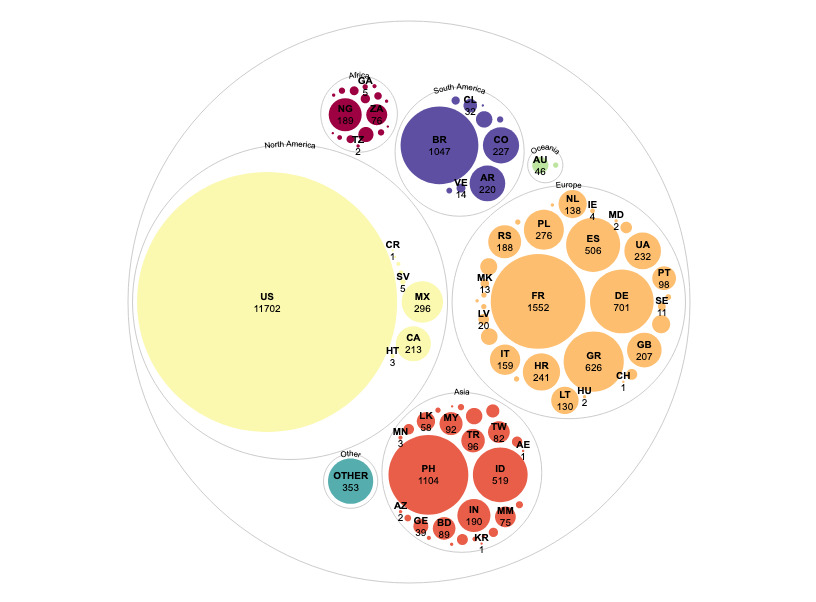
\includegraphics[scale = 0.5]{../img/viz_test.jpg}
\caption{Number of links ``fact checked as false" in the Condor Dataset, by country where it was most shared (`public\_shares\_top\_country").}
\end{figure}
\subsection*{illustrations ... }
\begin{enumerate}
	\item pie chart, number of youtube videos within set : available vs deleted
	\item Tweets: soft intervention 13 tweets, possibly sensitive 4\%, median/average follower count of the users who created the 13 tweets. what else ? 
	\item Facebook: reduced visibility graph - self-declared groups? but not from the set 
\end{enumerate}
Hence, in the present policy brief we explain how to verify  mainstream platforms' current actions regarding content with low credibility or false information with data mining. We do so by providing a series of examples for different interventions and platforms. We chose to focus on three platforms: Facebook, Twitter and YouTube. Both Facebook and YouTube are in the top three most popular social media platforms in terms of number of users.\footnote{See for example the ranking of the most popular social networks as of April 2021 on Statista: \href{https://www.statista.com/statistics/272014/global-social-networks-ranked-by-number-of-users/}{https://www.statista.com/statistics/272014/global-social-networks-ranked-by-number-of-users/}.} We further choose Twitter because it is a social networking platform with the most news-focused users, according to the Pew Research center (2019)~\cite{pew1}. To collect data from these three platforms, we either used the APIs (Application Programming Interfaces), or web scraping, i.e. retro-engineering the HMTL code of a web page to extract meaningful data, see Table \ref{tab1} for a summary. Minet \cite{minet}, a webmining tool developed by the SciencesPo médialab, was often used, and we scripted our own data mining code when it was necessary.

In this article we have assessed three broad categories of interventions to tackle misinformation by Facebook, Twitter and YouTube: $(i)$ suspension of accounts, $(ii)$ introduction of flags, labels and information panels and $(iii)$ reducing the visibility of content.\footnote{For a detailed list of interventions of multiple platforms, we invite the reader to navigate through the following \href{https://airtable.com/shrO0ooI9WSEfIUhb/tblAWQwFOiihKdQjm/viwZLAOzLK1NQ0c2n?blocks=hide}{airtable} compiled by Slatz and Leibowicz (2021)~\cite{niemanlab}.}
Furthermore, we have provided a methodology that can be useful for third-party monitoring. 
The code needed to collect the data and create the figures is available on the following public GitHub repository: \href{https://github.com/medialab/truth-and-trust-online-2021/}{https://github.com/medialab/truth-and-trust-online-2021/}, and we hope it can be a useful ressource for researchers, NGOs and journalists addressing online misinformation. 


\begin{table}[h]
\centering
\begin{tabular}{|l|c|l|l|l}

\hline
&  \begin{tabular}[c]{@{}l@{}} Application Programming Interface (API)  \end{tabular}                                                                                                                                                                                                                                                                                                                                                                                                                                            &    \multicolumn{1}{l|}{\begin{tabular}[c]{@{}l@{}} Web Scraping \end{tabular}}                                                                                                                                                                 \\ \hline
 
\includegraphics[scale=0.05]{../img/fb_logo.png} & \begin{tabular}[c]{@{}l@{}}\href{https://www.crowdtangle.com}{CrowdTangle API} and  \href{https://buzzsumo.com}{Buzzsumo API}   \end{tabular}                                                                                                                                                                                                               &      \multicolumn{1}{l|}{Code created for this article}    
\\ \hline
 
\includegraphics[scale=0.007]{../img/tw_logo.png}  &  \href{https://developer.twitter.com/en/docs/twitter-api/early-access}{Twitter API v2} & \multicolumn{1}{l|}{\href{https://github.com/medialab/minet/blob/master/docs/cli.md\#twitter-scrape}{Minet tw scrape}}                                                                                                                                                                           \\ \hline
 
\includegraphics[scale=0.03]{../img/yt_logo.png}  &  \href{https://developers.google.com/youtube/v3}{YouTube API v3}      &                                                                                                                            \multicolumn{1}{l|}{Code created for this article}                                                                                                                                                                           \\ \hline
\end{tabular}
\caption{Summary of ressources used for data collection.}
\label{tab1}
\end{table}

\smallskip

\subsection*{Notational variants}

We are aware that full transparency regarding operational aspects of misinformation related interventions can backfire.
This is because the aimed users might find means to circumvent the interventions. 
We noticed that some YouTube channels are trying to avoid the likely automated COVID-19 information panels, by using notational variants such as ``C.O.V.I.D'' or ``C O V I D''. 
Similarly, we came across notational variants on Twitter of the domain name {\it off-guardian.org}
\footnote{Here is an example of a failed fact-check of one of the articles of the website {\it off-guardian.org} : \href{https://www.politifact.com/factchecks/2020/jul/07/blog-posting/covid-19-tests-are-not-scientifically-meaningless/}{politifact.com/factchecks/2020/jul/07/blog-posting/covid-19-tests-are-not-scientifically-meaningless/}}
such as {\it off-guardian. org}, {\it off-guardian .org}, {\it off-guardian./org}, {\it off-guardian*org}.\footnote{For this case, we failed to understand precisely what kind of intervention Twitter users were circumventing, since they could share in a Tweet an article redirecting to the website {\it off-guardian.org} with the correct notation and only a warning message would appear when one clicks on it.}

\section{What should policy makers and digital platforms do?}

\begin{enumerate}
	\item For monitoring and auditing tasks, {\bf give access via main APIs, to deleted content due to policy violations} and specify the reason. 
	\smallskip
	
	Digital platform can remove content that violates their rules or or invite users to delete it themselves via a notification to regain access to the functionalities of their account. In both cases, the data can no longer be accessed via scraping or via the official APIs (Twitter, YouTube, CrowdTangle) for the purposes of scientific research. This hampers the investigation of which content is moderated and why. Moreover data can disappear from platforms over time (see Mazoyer et al. 2020~\cite{mazoyer2020french}), hence it is hard to distinguish whether platforms or users are the ones responsible for data removal.
	\item For monitoring and auditing tasks, {\bf give access via main APIs to essential metrics, such as:}
		\begin{enumerate} \setlength\itemsep{1em}
			\item a field indicating the {\bf {``reach"} of posts on Facebook.} \smallskip
			
			 The number of people who actually see a given post, cannot be recovered from the CrowdTangle API.\footnote{See \href{https://help.crowdtangle.com/en/articles/4558716-understanding-and-citing-crowdtangle-data}{https://help.crowdtangle.com/en/articles/4558716-understanding-and-citing-crowdtangle-data}.} Hence, researchers can only build proxies for this metric based on available data.
			\item a field indicating the {\bf policy violation leading to account suspension} on Twitter, Youtube and Facebook, and the content itself that led to that decision.  
			
			\item  a field indicating {\bf the presence of a banner, an information panel, a notice.}  \smallskip 
			
			To the best of our knowledge, fields related to flags, notices and information panels are not available on the official APIs, with the exception of the {\it withheld}  and {\it possibly sensitive content} interstitials in the Twitter API v2. 
			\item a field indicating whether {\bf content was signaled and how many times.}
			\item a field indicating the {\bf number of strikes received by an account} (Twitter, Facebook, Youtube) along with the content that caused the strike.
		\end{enumerate}

\item {\bf Allow the access to more data - Facebook Crowdtangle}

\smallskip

There is a growing restrictions to access APIs (Perriam et al.(2019)~\cite{api}).
In April $2018$, Facebook severely limited access to their official APIs\footnote{See \href{https://about.fb.com/news/2018/04/restricting-data-access/}{https://about.fb.com/news/2018/04/restricting-data-access/} and \href{http://thepoliticsofsystems.net/2018/08/facebooks-app-review-and-how-independent-research-just-got-a-lot-harder/}{http://thepoliticsofsystems.net/2018/08/} \href{http://thepoliticsofsystems.net/2018/08/facebooks-app-review-and-how-independent-research-just-got-a-lot-harder/}{/facebooks-app-review-and-how-independent-research-just-got-a-lot-harder/}.} 
and CrowdTangle is today a reliable source for researchers to access Facebook data. 
However, it should be noted that CrowdTangle has been recently used by journalists to show that Facebook is spreading biased information\footnote{See the news article \href{https://www.economist.com/graphic-detail/2020/09/10/facebook-offers-a-distorted-view-of-american-news}{https://www.economist.com/graphic-detail/2020/09/10/facebook-offers-a-distorted-view-of-american-news} and the tweet \href{https://twitter.com/facebookstop10}{https://twitter.com/facebookstop10}. 
The last link is a Twitter account showing each day the ten most shared link on Facebook, most of them coming from extreme right and misinformation sources. 
Facebook has reacted to this here: \href{https://about.fb.com/news/2020/11/what-do-people-actually-see-on-facebook-in-the-us/}{https://about.fb.com/news/2020/11/what-do-people-actually-see-on-facebook-in-the-us/}.} 
and a general suspicion is growing that its access might be shut down in a near future to journalists and researchers.\footnote{See the news articles \href{https://www.nytimes.com/2021/07/14/technology/facebook-data.html}{https://www.nytimes.com/2021/07/14/technology/facebook-data.html} and \href{https://www.bloomberg.com/news/articles/2021-08-03/facebook-disables-accounts-tied-to-nyu-research-project}{https://www.bloomberg.com/news/articles/2021-08-03/facebook-disables-accounts-tied-to-nyu-research-project}.}

Regarding Twitter and YouTube, it is still possible and relatively easy to access their official APIs. Nevertheless the number of Tweets that can be retrieved has decreased between the Twitter API v1 and v2. 
In the v2, there is a monthly cap of $10,000,000$ Tweets for the academic research track\footnote{https://developer.twitter.com/en/docs/projects/overview},
while in the v1 there was no monthly limit and only a limit on the number of requests that could be made in a 15-minute window\footnote{https://developer.twitter.com/en/docs/twitter-api/v1/rate-limits}.
We thus noticed that we could get around $10$ times more Tweets per month with the v1 when compared to the v2 for one specific collection.

\smallskip

Number of articles on google scholar showing disproportionate access when compared to the size of the platform: 
\begin{itemize}
	\item Twitter (all time) : about 7,830,000 results (0.19 sec)
	\item Facebook (all time) : about 7,040,000 results (0.06 sec)
	\item Youtube (all time) : about 6,520,000 results (0.03 sec)
	\item Telegram (all time, possible mistakes): about 5,970 results (0.02 sec)
\end{itemize}
\item {\bf Enrich transparency reports with a specific section for misinformation interventions + cross categories }
\smallskip

When navigating through the categories of policy areas, to the best of our knowledge, misinformation is absent from the data available on the transparency centers of Facebook, Twitter and YouTube. Platforms' official communication about misinformation interventions is scarce and the academic community, NGOs and data journalists, usually discover interventions related to misinformation via monitoring social media accounts related to domain names with several failed fact-checks or via articles in News outlets. 

\smallskip

In certain cases, the platform interventions were not motivated by content moderation to limit misinformation, but rather by other rule violations. For example, the official reason for the suspension of Donald Trump's Twitter account was not misinformation\footnote{Although Donald Trump may have spread many misinformation during his governance, see for example: \href{http://allianceforscience.cornell.edu/blog/2020/10/what-drove-the-covid-misinformation-infodemic/}{http://allianceforscience.cornell.edu/blog/2020/10/what-drove-the-covid-misinformation-infodemic/}.}
but the violation of Twitter's Glorification of Violence Policy, with his last tweets encouraging the Capitol's riot.\footnote{See \href{https://blog.twitter.com/en\_us/topics/company/2020/suspension}{https://blog.twitter.com/en\_us/topics/company/2020/suspension}.} Similarly, when Facebook removed four pages related to the InfoWars website, the cited reason was repeated violations of Community Standards: 
``While much of the discussion around Infowars has been related to false news, which is a serious issue that we are working to address [...], none of the violations that spurred today’s removals were related to this''.\footnote{See the article \href{https://about.fb.com/news/2018/08/enforcing-our-community-standards/}{https://about.fb.com/news/2018/08/enforcing-our-community-standards/}.}
Regarding The Beauty of Life website, its ban was officially due to coordinated inauthentic behavior,\footnote{See \href{https://about.fb.com/news/2019/12/removing-coordinated-inauthentic-behavior-from-georgia-vietnam-and-the-us/}{https://about.fb.com/news/2019/12/removing-coordinated-inauthentic-behavior-from-georgia-vietnam-and-the-us/}.} 
which includes using fake accounts that misrepresent one's identity or using methods to artificially boost the popularity of content. 
According to Facebook, coordinated inauthentic behavior is a distinct phenomenon from disinformation, as ``most of the content shared by coordinated manipulation campaigns isn’t probably false''.\footnote{See: \href{https://about.fb.com/news/2019/10/inauthentic-behavior-policy-update/}{https://about.fb.com/news/2019/10/inauthentic-behavior-policy-update/}.} 
Nevertheless, both misinformation and coordinated inauthentic behavior were attested for the Beauty of Life, and reported to Facebook by the fact-checking organization Snopes.\footnote{See \href{ https://www.snopes.com/news/2019/11/12/bl-fake-profiles/}{https://www.snopes.com/news/2019/11/12/bl-fake-profiles/}, 
\href{https://www.snopes.com/news/2019/11/12/bl-fake-profiles/}{https://www.snopes.com/news/2019/11/12/bl-} \href{https://www.snopes.com/news/2019/11/12/bl-fake-profiles/}{fake-profiles/}  and 
\href{https://www.snopes.com/news/2019/12/13/facebook-bl-cib/}{https://www.snopes.com/news/2019/12/13/facebook-bl-cib/}.} 
Because misinformation is often associated with creating fake accounts to speed its spread, and incitation to violence, it is sometimes unclear to distinguish between interventions due to misinformation and interventions due to other guideline violations, and more transparent communication on platforms' actions would help monitor the interventions specifically related to misinformation.
\smallskip

Furthermore, it is likely that most interventions used to tackle online misinformation correspond to interventions that were designed for earlier policy areas.
To illustrate, YouTube explicitly states
\footnote{See {\it What policies exist to fight misinformation on Youtube?} \href{https://www.youtube.com/intl/en\_us/howyoutubeworks/our-commitments/fighting-misinformation/\#policies}{youtube.com/intl/en\_us/howyoutubeworks/our-commitments/fighting-misinformation/\#policies}.}
that: ``Several policies in our Community Guidelines are directly applicable to misinformation'', such as the deceptive practices, impersonation and hate speech policies.
Hence interventions such as content deletion or account suspension, might be efficient for policy areas for which they were specifically designed, such as the policy area {\it Adult Nudity \& Sexual Activity}. Nevertheless, tackling online misinformation might need adapted interventions.
Namely, account suspensions or content deletion motivated by the spread of inaccurate information can be perceived as censorship by the targeted users. In particular, such interventions can generate platform migrations towards new alternative social media platforms (e.g. Telegram, Gab, Minds) with little or no content moderation (see Rogers (2020)~\cite{rogers2020}).

\item {\bf Specific API for monitoring and auditing and the study of misinformation in general and relevance of policies}

Moreover, a fact-checking label can lead to unpredicted consequences depending on the perception of the person reading it.
On Facebook, Twitter and YouTube, fact-checking messages are currently applied only to some content, while the rest of the content on a given platform remains naturally unlabelled. 
Such sparse application of warnings can lead to an ``implied truth'' effect, where users may assume that content without warnings have actually been verified and shown to be true (Pennycook et al. (2020)~\cite{pennycook2020implied}).
Using a different approach, Mosleh et al. (2021)~\cite{mosleh2021perverse} identified Twitter users sharing false news and replied to their false tweets with links redirecting to fact-checking websites.
They observed a decrease in the quality and accuracy of the content subsequently shared by the corrected user. 
These research papers highlight the necessity to investigate potential unintended effects of well-meaning interventions.
The methods presented in this paper can help to monitor not only the platforms' actions against misinformation, but also their subsequent consequences in real-life settings.

\end{enumerate}


\section{Quick access to community guidelines and platform misinformation policies} \label{links}


\begin{landscape}

\thispagestyle{empty}

\begin{table}[p]
\centering
\setlength{\tabcolsep}{2pt}
\begin{tabular}{|c|c|c|}
\hline
\multirow{3}{*}{Rules}                     & 
\includegraphics[scale=0.05]{./img/fb_logo.png} & \begin{tabular}[c]{@{}cl@{}}   \href{https://www.facebook.com/communitystandards/recentupdates/}{facebook.com/communitystandards/recentupdates/}    \end{tabular}                     \\ \cline{2-3} 
                                           & 
\includegraphics[scale=0.007]{./img/tw_logo.png}   & \href{https://help.twitter.com/en/rules-and-policies/twitter-rules}{help.twitter.com/en/rules-and-policies/twitter-rules}                       \\ \cline{2-3} 
                                           & 
\includegraphics[scale=0.03]{./img/yt_logo.png}  & \href{https://www.youtube.com/intl/en\_us/howyoutubeworks/policies/community-guidelines/}{youtube.com/intl/en\_us/howyoutubeworks/policies/community-guidelines/} \\ \hline
\multirow{3}{*}{\begin{tabular}[c]{@{}cl@{}}  Rules \\ enforcement \end{tabular}}         & 
\includegraphics[scale=0.05]{./img/fb_logo.png}  & \href{https://transparency.fb.com/data/community-standards-enforcement/}{transparency.fb.com/data/community-standards-enforcement/}                 \\ \cline{2-3} 
                                           & 
\includegraphics[scale=0.007]{./img/tw_logo.png}   & \href{https://transparency.twitter.com/en/reports/rules-enforcement.html}{transparency.twitter.com/en/reports/rules-enforcement.html}                \\ \cline{2-3} 
                                           & 
\includegraphics[scale=0.03]{./img/yt_logo.png}  & \href{https://transparencyreport.google.com/youtube-policy/}{transparencyreport.google.com/youtube-policy/}                              \\ \hline
\multirow{3}{*}{\begin{tabular}[c]{@{}cl@{}}  Transparency \\ center \end{tabular}}       & 
\includegraphics[scale=0.05]{./img/fb_logo.png} & \begin{tabular}[c]{@{}cl@{}}  \href{https://transparency.fb.com/data/}{transparency.fb.com/data/}    \\ \href{https://law.yale.edu/yls-today/news/facebook-data-transparency-advisory-group-releases-final-report}{https://law.yale.edu/yls-today/news/facebook-data-transparency-advisory-group-releases-final-report} \end{tabular}                                               \\ \cline{2-3} 
                                           & 
\includegraphics[scale=0.007]{./img/tw_logo.png}   & \href{https://transparency.twitter.com/en/reports.html}{transparency.twitter.com/en/reports.html}                                  \\ \cline{2-3} 
                                           & 
\includegraphics[scale=0.03]{./img/yt_logo.png}  & \href{https://transparencyreport.google.com/?hl=en}{transparencyreport.google.com/?hl=en}                                      \\ \hline
\multirow{3}{*}{\begin{tabular}[c]{@{}cl@{}}  Policy \\ regarding \\  Covid-19 \end{tabular}} & 
\includegraphics[scale=0.05]{./img/fb_logo.png} & https://www.facebook.com/help/230764881494641/                                     \\ \cline{2-3} 
                                           & 
\includegraphics[scale=0.007]{./img/tw_logo.png}   & \begin{tabular}[c]{@{}cl@{}} \href{https://help.twitter.com/en/rules-and-policies/medical-misinformation-policy}{help.twitter.com/en/rules-and-policies/medical-misinformation-policy} \\  \href{https://blog.twitter.com/en\_us/topics/company/2021/updates-to-our-work-on-covid-19-vaccine-misinformation}{blog.twitter.com/en\_us/topics/company/2021/updates-to-our-work-on-covid-19-vaccine-misinformation} \\  \href{https://blog.twitter.com/en\_us/topics/company/2020/covid-19}{blog.twitter.com/en\_us/topics/company/2020/covid-19}\end{tabular}      \\ \cline{2-3} 
                                           & 
\includegraphics[scale=0.03]{./img/yt_logo.png}  & \href{https://support.google.com/youtube/answer/9891785}{support.google.com/youtube/answer/9891785}                                 \\ \hline
\multirow{3}{*}{\begin{tabular}[c]{@{}cl@{}}  Fact-checking \\ policy \end{tabular}} & 
\includegraphics[scale=0.05]{./img/fb_logo.png} & \href{https://www.facebook.com/journalismproject/programs/third-party-fact-checking/how-it-works}{facebook.com/journalismproject/programs/third-party-fact-checking/how-it-works}                                    \\ \cline{2-3} 
                                           & 
\includegraphics[scale=0.007]{./img/tw_logo.png}   & x       \\ \cline{2-3} 
                                           & 
\includegraphics[scale=0.03]{./img/yt_logo.png}  & \href{https://support.google.com/youtube/answer/9229632}{support.google.com/youtube/answer/9229632}                                  \\ \hline
\multirow{3}{*}{\begin{tabular}[c]{@{}cl@{}}  Fighting \\ misinformation \end{tabular}} & 
\includegraphics[scale=0.05]{./img/fb_logo.png} & \begin{tabular}[c]{@{}cl@{}} \href{https://www.facebook.com/formedia/blog/working-to-stop-misinformation-and-false-news}{facebook.com/formedia/blog/working-to-stop-misinformation-and-false-news}     \\ \href{https://about.fb.com/news/2018/05/hard-questions-false-news/}{about.fb.com/news/2018/05/hard-questions-false-news/}   \end{tabular}                            \\ \cline{2-3} 
                                           & 
\includegraphics[scale=0.007]{./img/tw_logo.png}   &        \\ \cline{2-3} 
                                           & 
\includegraphics[scale=0.03]{./img/yt_logo.png}  & \begin{tabular}[c]{@{}cl@{}}  \href{https://www.youtube.com/intl/en\_us/howyoutubeworks/our-commitments/fighting-misinformation/\#policies}{youtube.com/intl/en\_us/howyoutubeworks/our-commitments/fighting-misinformation/\#policies}  \\ \href{https://blog.youtube/inside-youtube/the-four-rs-of-responsibility-raise-and-reduce/}{blog.youtube/inside-youtube/the-four-rs-of-responsibility-raise-and-reduce/}    \end{tabular}                            \\ \hline
                                           
% 

\multirow{3}{*}{\begin{tabular}[c]{@{}cl@{}} Strike System \end{tabular}} & 
\includegraphics[scale=0.05]{./img/fb_logo.png} & \begin{tabular}[c]{@{}cl@{}} See in the following link the section {\it What is the number of strikes a person or } \\ { \it Page has to get to before you ban them?} \\  \href{https://about.fb.com/news/2018/08/enforcing-our-community-standards/}{about.fb.com/news/2018/08/enforcing-our-community-standards/} \\ \href{https://transparency.fb.com/en-gb/enforcement/taking-action/counting-strikes/}{https://transparency.fb.com/en-gb/enforcement/taking-action/counting-strikes/} (updated July 29,2021)   \end{tabular}                            \\ \cline{2-3} 
                                           & 
\includegraphics[scale=0.007]{./img/tw_logo.png}   &  \begin{tabular}[c]{@{}cl@{}}  See in the following links the section:  {\it Account locks and permanent suspension }   \\ \href{https://help.twitter.com/en/rules-and-policies/election-integrity-policy}{help.twitter.com/en/rules-and-policies/election-integrity-policy}  \\ \href{https://help.twitter.com/en/rules-and-policies/medical-misinformation-policy}{help.twitter.com/en/rules-and-policies/medical-misinformation-policy}  \end{tabular}    \\ \cline{2-3} 
                                           & 
\includegraphics[scale=0.03]{./img/yt_logo.png}  & \begin{tabular}[c]{@{}cl@{}}  \href{https://support.google.com/youtube/answer/2802032?hl=en. Accessed 21 6 2021}{https://support.google.com/youtube/answer/2802032?hl=en. Accessed 21 6 2021}   \end{tabular}                            \\ \hline 

% 

\multirow{3}{*}{\begin{tabular}[c]{@{}cl@{}} Account suspension \end{tabular}} & 
\includegraphics[scale=0.05]{./img/fb_logo.png} & \begin{tabular}[c]{@{}cl@{}}    \end{tabular}                            \\ \cline{2-3} 
                                           & 
\includegraphics[scale=0.007]{./img/tw_logo.png}   &  \begin{tabular}[c]{@{}cl@{}} \href{https://help.twitter.com/en/managing-your-account/suspended-twitter-accounts}{https://help.twitter.com/en/managing-your-account/suspended-twitter-accounts }    \end{tabular}    \\ \cline{2-3} 
                                           & 
\includegraphics[scale=0.03]{./img/yt_logo.png}  & \begin{tabular}[c]{@{}cl@{}}    \end{tabular}                            \\ \hline                                            

% 

\multirow{3}{*}{\begin{tabular}[c]{@{}cl@{}} Flags, Notice \\ and Information Panels \end{tabular}} & 
\includegraphics[scale=0.05]{./img/fb_logo.png} & \begin{tabular}[c]{@{}cl@{}}  \href{https://www.facebook.com/business/help/341102040382165}{https://www.facebook.com/business/help/341102040382165}   \end{tabular}                            \\ \cline{2-3} 
                                           & 
\includegraphics[scale=0.007]{./img/tw_logo.png}   &  \begin{tabular}[c]{@{}cl@{}} \href{https://help.twitter.com/en/rules-and-policies/notices-on-twitter}{https://help.twitter.com/en/rules-and-policies/notices-on-twitter}    \end{tabular}    \\ \cline{2-3} 
                                           & 
\includegraphics[scale=0.03]{./img/yt_logo.png}  & \begin{tabular}[c]{@{}cl@{}}   \href{https://support.google.com/youtube/answer/9004474?hl=en}{support.google.com/youtube/answer/9004474?hl=en}  \end{tabular}                            \\ \hline
                                                                                  
 \end{tabular}
\caption{Summary of ressources, last accessed on July 5, 2021. }
\label{summary}
\end{table}

\end{landscape}

\section*{Further reading}

\begin{itemize}
	\item 
\end{itemize}

\bibliography{proj1}{}
\bibliographystyle{plain}



\end{document}